% Options for packages loaded elsewhere
\PassOptionsToPackage{unicode}{hyperref}
\PassOptionsToPackage{hyphens}{url}
%
\documentclass[
  ignorenonframetext,
]{beamer}
\usepackage{pgfpages}
\setbeamertemplate{caption}[numbered]
\setbeamertemplate{caption label separator}{: }
\setbeamercolor{caption name}{fg=normal text.fg}
\beamertemplatenavigationsymbolshorizontal
% Prevent slide breaks in the middle of a paragraph
\widowpenalties 1 10000
\raggedbottom
\setbeamertemplate{part page}{
  \centering
  \begin{beamercolorbox}[sep=16pt,center]{part title}
    \usebeamerfont{part title}\insertpart\par
  \end{beamercolorbox}
}
\setbeamertemplate{section page}{
  \centering
  \begin{beamercolorbox}[sep=12pt,center]{part title}
    \usebeamerfont{section title}\insertsection\par
  \end{beamercolorbox}
}
\setbeamertemplate{subsection page}{
  \centering
  \begin{beamercolorbox}[sep=8pt,center]{part title}
    \usebeamerfont{subsection title}\insertsubsection\par
  \end{beamercolorbox}
}
\AtBeginPart{
  \frame{\partpage}
}
\AtBeginSection{
  \ifbibliography
  \else
    \frame{\sectionpage}
  \fi
}
\AtBeginSubsection{
  \frame{\subsectionpage}
}

\usepackage{amsmath,amssymb}
\usepackage{iftex}
\ifPDFTeX
  \usepackage[T1]{fontenc}
  \usepackage[utf8]{inputenc}
  \usepackage{textcomp} % provide euro and other symbols
\else % if luatex or xetex
  \usepackage{unicode-math}
  \defaultfontfeatures{Scale=MatchLowercase}
  \defaultfontfeatures[\rmfamily]{Ligatures=TeX,Scale=1}
\fi
\usepackage{lmodern}
\usetheme[]{default}
\ifPDFTeX\else  
    % xetex/luatex font selection
\fi
% Use upquote if available, for straight quotes in verbatim environments
\IfFileExists{upquote.sty}{\usepackage{upquote}}{}
\IfFileExists{microtype.sty}{% use microtype if available
  \usepackage[]{microtype}
  \UseMicrotypeSet[protrusion]{basicmath} % disable protrusion for tt fonts
}{}
\makeatletter
\@ifundefined{KOMAClassName}{% if non-KOMA class
  \IfFileExists{parskip.sty}{%
    \usepackage{parskip}
  }{% else
    \setlength{\parindent}{0pt}
    \setlength{\parskip}{6pt plus 2pt minus 1pt}}
}{% if KOMA class
  \KOMAoptions{parskip=half}}
\makeatother
\usepackage{xcolor}
\newif\ifbibliography
\setlength{\emergencystretch}{3em} % prevent overfull lines
\setcounter{secnumdepth}{-\maxdimen} % remove section numbering


\providecommand{\tightlist}{%
  \setlength{\itemsep}{0pt}\setlength{\parskip}{0pt}}\usepackage{longtable,booktabs,array}
\usepackage{calc} % for calculating minipage widths
\usepackage{caption}
% Make caption package work with longtable
\makeatletter
\def\fnum@table{\tablename~\thetable}
\makeatother
\usepackage{graphicx}
\makeatletter
\def\maxwidth{\ifdim\Gin@nat@width>\linewidth\linewidth\else\Gin@nat@width\fi}
\def\maxheight{\ifdim\Gin@nat@height>\textheight\textheight\else\Gin@nat@height\fi}
\makeatother
% Scale images if necessary, so that they will not overflow the page
% margins by default, and it is still possible to overwrite the defaults
% using explicit options in \includegraphics[width, height, ...]{}
\setkeys{Gin}{width=\maxwidth,height=\maxheight,keepaspectratio}
% Set default figure placement to htbp
\makeatletter
\def\fps@figure{htbp}
\makeatother

\usepackage{booktabs}
\usepackage{longtable}
\usepackage{array}
\usepackage{multirow}
\usepackage{wrapfig}
\usepackage{float}
\usepackage{colortbl}
\usepackage{pdflscape}
\usepackage{tabu}
\usepackage{threeparttable}
\usepackage{threeparttablex}
\usepackage[normalem]{ulem}
\usepackage{makecell}
\usepackage{xcolor}
\newcommand{\theHtable}{\thetable}
\makeatletter
\@ifpackageloaded{caption}{}{\usepackage{caption}}
\AtBeginDocument{%
\ifdefined\contentsname
  \renewcommand*\contentsname{Table of contents}
\else
  \newcommand\contentsname{Table of contents}
\fi
\ifdefined\listfigurename
  \renewcommand*\listfigurename{List of Figures}
\else
  \newcommand\listfigurename{List of Figures}
\fi
\ifdefined\listtablename
  \renewcommand*\listtablename{List of Tables}
\else
  \newcommand\listtablename{List of Tables}
\fi
\ifdefined\figurename
  \renewcommand*\figurename{Figure}
\else
  \newcommand\figurename{Figure}
\fi
\ifdefined\tablename
  \renewcommand*\tablename{Table}
\else
  \newcommand\tablename{Table}
\fi
}
\@ifpackageloaded{float}{}{\usepackage{float}}
\floatstyle{ruled}
\@ifundefined{c@chapter}{\newfloat{codelisting}{h}{lop}}{\newfloat{codelisting}{h}{lop}[chapter]}
\floatname{codelisting}{Listing}
\newcommand*\listoflistings{\listof{codelisting}{List of Listings}}
\makeatother
\makeatletter
\makeatother
\makeatletter
\@ifpackageloaded{caption}{}{\usepackage{caption}}
\@ifpackageloaded{subcaption}{}{\usepackage{subcaption}}
\makeatother
\ifLuaTeX
  \usepackage{selnolig}  % disable illegal ligatures
\fi
\usepackage{bookmark}

\IfFileExists{xurl.sty}{\usepackage{xurl}}{} % add URL line breaks if available
\urlstyle{same} % disable monospaced font for URLs
\hypersetup{
  pdftitle={Class 10},
  pdfauthor={Sarah E. Grabinski},
  hidelinks,
  pdfcreator={LaTeX via pandoc}}

\title{Class 10}
\subtitle{DATA1220-55, Fall 2024}
\author{Sarah E. Grabinski}
\date{2024-09-20}

\begin{document}
\frame{\titlepage}

\begin{frame}[fragile]{Homework 2}
\phantomsection\label{homework-2}
\begin{itemize}
\item
  \href{https://canvas.jcu.edu/files/3708401/download?download_frd=1}{Instructions}
  (\texttt{homework2\_instructions.pdf}), a
  \href{https://canvas.jcu.edu/files/3708307/download?download_frd=1}{Quarto
  markdown template} (\texttt{homework2\_template.qmd}), and an
  \href{https://canvas.jcu.edu/files/3708306/download?download_frd=1}{example
  HTML output} (\texttt{homework2\_example.html}) are available for
  download under Chapter 2 on the
  \href{https://canvas.jcu.edu/courses/36290/modules}{Modules} page in
  Canvas.
\item
  \href{https://canvas.jcu.edu/files/3708369/download?download_frd=1}{Video
  walk-through} of Homework 2 under Tutorials on the Modules page in
  Canvas. Make sure you're caught up on the
  \href{https://canvas.jcu.edu/files/3695568/download?download_frd=1}{video
  walk-through of homework 1}.
\item
  Upload \textbf{\emph{TWO}} (2) documents to
  \href{https://canvas.jcu.edu/courses/36290/assignments/451733}{Homework
  2} on the
  \href{https://canvas.jcu.edu/courses/36290/assignments}{Assignments}
  page in Canvas by Friday 9/20/2024 by 6:00pm:
  \texttt{homework2\_yourlastname.qmd} and
  \texttt{homework2\_yourlastname.html}
\end{itemize}
\end{frame}

\begin{frame}{Homework Hints}
\phantomsection\label{homework-hints}
\begin{itemize}
\item
  \emph{Read the instructions!} Some of the issues you're having are
  because you did not follow them correctly.
\item
  \emph{Please answer in complete sentences where possible!} I want you
  to practice effectively communicating data, and life is not a multiple
  choice question. I will be more clear about indicating this on future
  homework.
\item
  Real world distributions are harder to describe than idealized
  theoretical distributions. \emph{Combining visual and numeric
  summaries is more powerful than using either alone.}
\end{itemize}
\end{frame}

\begin{frame}{Campuswire Hints}
\phantomsection\label{campuswire-hints}
\begin{itemize}
\item
  \emph{Turn on notifications.} Your question may have already been
  asked and answered. Campuswire can email you when there are new posts,
  so you can keep up with the discussion.
\item
  \emph{Be specific!} A detailed question is more likely to get a
  (useful) answer than a general question.
\item
  \emph{Include code \& error messages.} It is much easier to
  troubleshoot ``My document won't render. I've copy-pasted the error
  message and the lines of code where it breaks.'' than ``My document
  won't render.'' \emph{Click
  \href{https://stackoverflow.com/help/minimal-reproducible-example}{here}
  for more info on how to ask good debugging questions.}
\end{itemize}
\end{frame}

\begin{frame}{How can I get help with homework?}
\phantomsection\label{how-can-i-get-help-with-homework}
\begin{itemize}
\item
  \textbf{Read the
  \href{https://canvas.jcu.edu/files/3669904/download?download_frd=1}{textbook}.}
  Many of you are asking for additional examples. Luckily, there are
  tons we didn't go over in the textbook.
\item
  \textbf{Ask a question on our
  \href{https://campuswire.com/c/G6427C531/feed}{Campuswire class
  feed}.} I'm only one person, and I may not be able to give you a
  prompt answer. However, the 20+ other people in the class might be
  able to.
\end{itemize}

\emph{I will try to keep an eye on Campuswire posts between 4-6pm before
the homework is due, but I have other things going on and might miss
something.}
\end{frame}

\begin{frame}{Last time\ldots{} defining probability}
\phantomsection\label{last-time-defining-probability}
\begin{itemize}
\item
  \textbf{\emph{Probability:}} The proportion of times that a particular
  outcome would occur if we observed a random process an infinite number
  of times (\(\operatorname{P}(\operatorname{Event = A})\).

  \begin{itemize}
  \item
    Ranges from 0 to 1 or 0\% to 100\%
  \item
    \(0 \le \operatorname{probability} \le 1\)
  \item
    Probability = Proportion
  \end{itemize}
\item
  \textbf{\emph{Random process:}} you know which outcomes are possible
  (i.e.~the \textbf{sample space}) but you don't know which outcome
  comes next
\end{itemize}
\end{frame}

\begin{frame}{Last time\ldots{} representing probability}
\phantomsection\label{last-time-representing-probability}
\begin{itemize}
\item
  \textbf{\emph{Sample space:}} all possible outcomes of a random
  process (\(S\))
\item
  \textbf{\emph{Disjoint events:}} events that CANNOT occur at the same
  time (\textbf{\emph{mutually exclusive}})
\item
  \textbf{\emph{Complement:}} the complement of any event \(A\) which
  exists in sample space \(S\) is any outcome also in sample space \(S\)
  which is NOT \(A\) (\(A^C\) or \(A'\))

  \begin{itemize}
  \item
    Complements are always disjoint
  \item
    The probability of event A occuring OR the complement of event A
    occuring is always 1
  \end{itemize}
\item
  \textbf{\emph{Non-disjoint events:}} events that CAN occur at the same
  time
\end{itemize}
\end{frame}

\begin{frame}{Last time\ldots{} calculating probabilities}
\phantomsection\label{last-time-calculating-probabilities}
Remember\ldots{}

\begin{itemize}
\item
  \(\operatorname{P}(S)=1\)
\item
  \(\operatorname{P}(S)=\operatorname{P}(A)+\operatorname{P}(A')\)
\item
  \(\operatorname{P}(A)+\operatorname{P}(A')=1\)
\item
  \(\operatorname{P}(A')=1-\operatorname{P}(A)\)
\end{itemize}
\end{frame}

\begin{frame}{Last time\ldots{} population probability}
\phantomsection\label{last-time-population-probability}
\begin{itemize}
\tightlist
\item
  \textbf{\emph{Population Probability:}} the theoretical ``true''
  probability of an outcome in the population of interest, the ``ground
  truth'' (\(p\))
\end{itemize}

\[
p=\frac{\operatorname{count}(\operatorname{events = A})}{\operatorname{count}(\operatorname{all events in sample space})}
\]
\end{frame}

\begin{frame}{Last time\ldots{} sample probability}
\phantomsection\label{last-time-sample-probability}
\begin{itemize}
\tightlist
\item
  \textbf{\emph{Sample Probability:}} the probability of an outcome
  observed in a sample of size \(n\) from a population with probability
  \(p\), an estimate of the population probability (\(\hat{p}_n\))
\end{itemize}

\[
\hat{p}_n=\frac{\operatorname{count}(\operatorname{observation = A})}{\operatorname{count}(\operatorname{observations in sample})}
\]
\end{frame}

\begin{frame}{Last time\ldots{} Law of Large Numbers}
\phantomsection\label{last-time-law-of-large-numbers}
\begin{columns}[T]
\begin{column}{0.48\textwidth}
\begin{itemize}
\item
  How well the sample proportion \(\hat{p}_n\) represents the population
  proportion \(p\) depends on the size of the denominator.
\item
  As more observations are collected, the sample proportion
  \(\hat{p}_n\) of a particular outcome approaches the population
  proportion \(p\) of that outcome.
\item
  \(\lim_{n\to\infty} \hat{p}_n = p\) (As \(n \to \infty\),
  \(\hat{p}_n \to p\))
\end{itemize}
\end{column}

\begin{column}{0.48\textwidth}
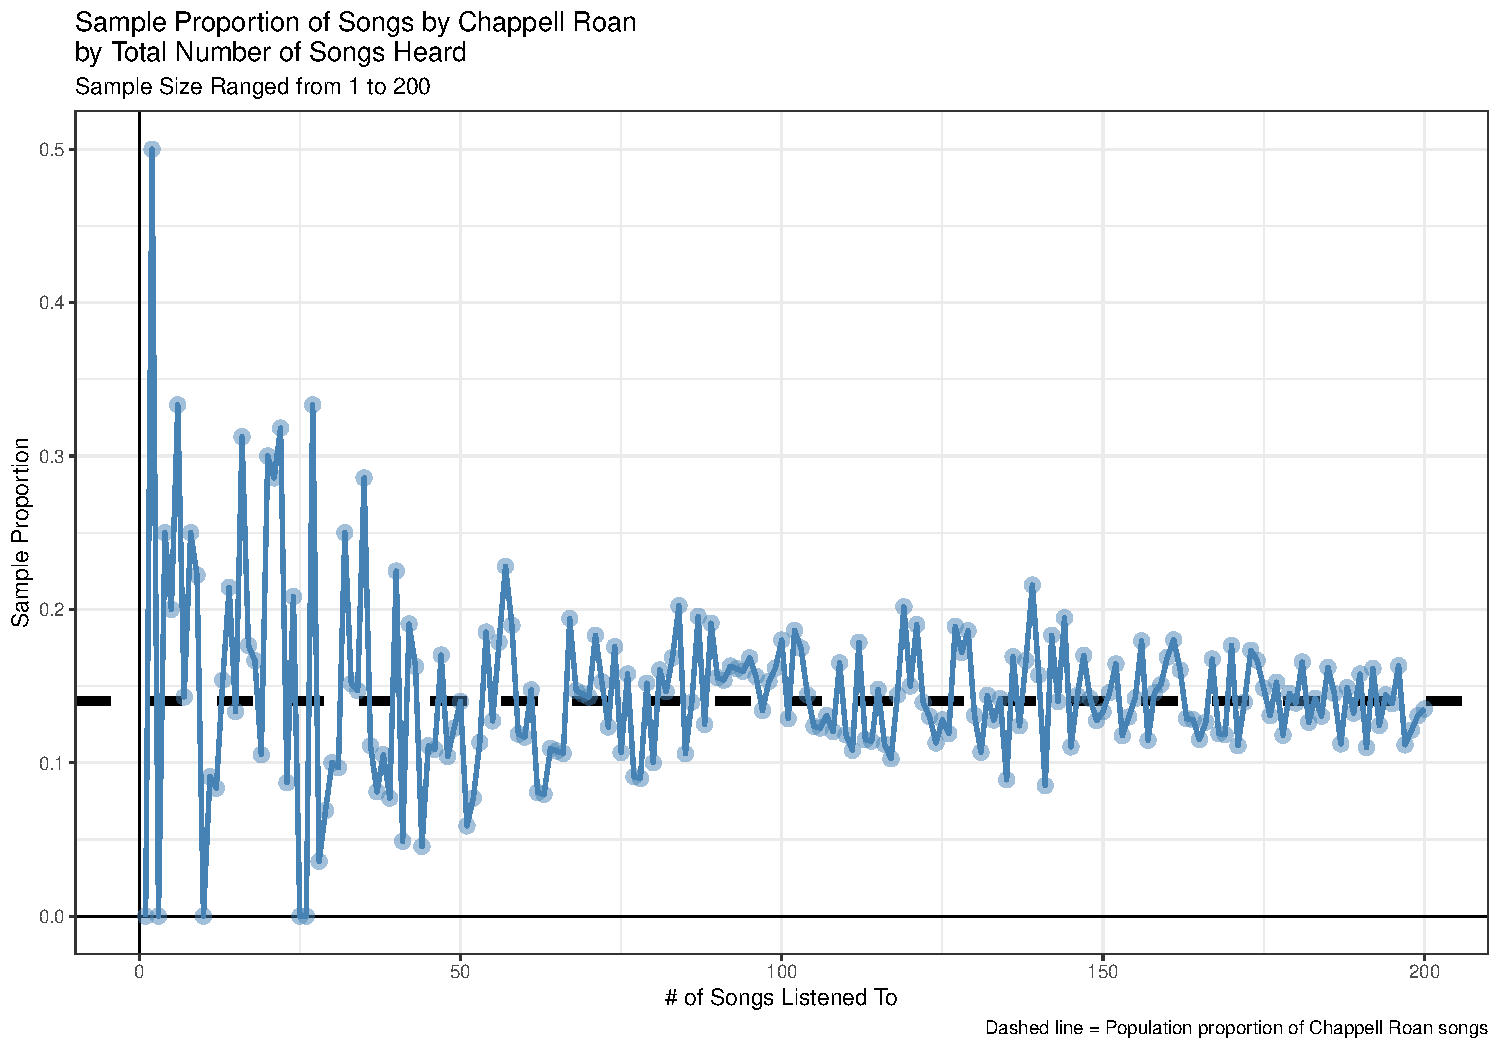
\includegraphics{class10_files/figure-beamer/unnamed-chunk-2-1.pdf}
\end{column}
\end{columns}
\end{frame}

\begin{frame}{Last time\ldots{} sampling WITH replacement}
\phantomsection\label{last-time-sampling-with-replacement}
\begin{figure}[H]

{\centering \includegraphics{class10_files/mediabag/Sampling-With-Replac.png}

}

\caption{\textbf{\emph{Sampling with replacement}} is like drawing a
card from a deck, then shuffling it back in before drawing another card.
Repetition is possible.}

\end{figure}%
\end{frame}

\begin{frame}{This time\ldots{}}
\phantomsection\label{this-time}
\begin{itemize}
\item
  Sampling WITHOUT replacement
\item
  Independent and dependent processes
\item
  Calculating probabilities for 2 events

  \begin{itemize}
  \item
    (General) Addition Rule
  \item
    (General) Multiplication Rule
  \end{itemize}
\item
  Probability distributions
\end{itemize}
\end{frame}

\begin{frame}{Returning to the playlist shuffle example\ldots{}}
\phantomsection\label{returning-to-the-playlist-shuffle-example}
\begin{itemize}
\item
  Extracted song names and artists from the ``Taylor Swift Radio''
  playlist on Spotify
\item
  There are 50 songs on the playlist by 26 different artists.
\item
  Some artists have more than 1 song on the playlist, and 1 song was a
  collaboration between 2 artists.
\item
  The iPod Shuffle originally used random sampling WITH replacement to
  select the next song to play (``true'' shuffle)
\item
  Spotify originally used random sampling WITHOUT replacement to select
  the next song to play (Fisher-Yates Algorithm)
\end{itemize}
\end{frame}

\begin{frame}{Let's define our sample space \(S\) again\ldots{}}
\phantomsection\label{lets-define-our-sample-space-s-again}
See board\ldots{}
\end{frame}

\begin{frame}{Population proportions by song for sampling WITH
replacement}
\phantomsection\label{population-proportions-by-song-for-sampling-with-replacement}
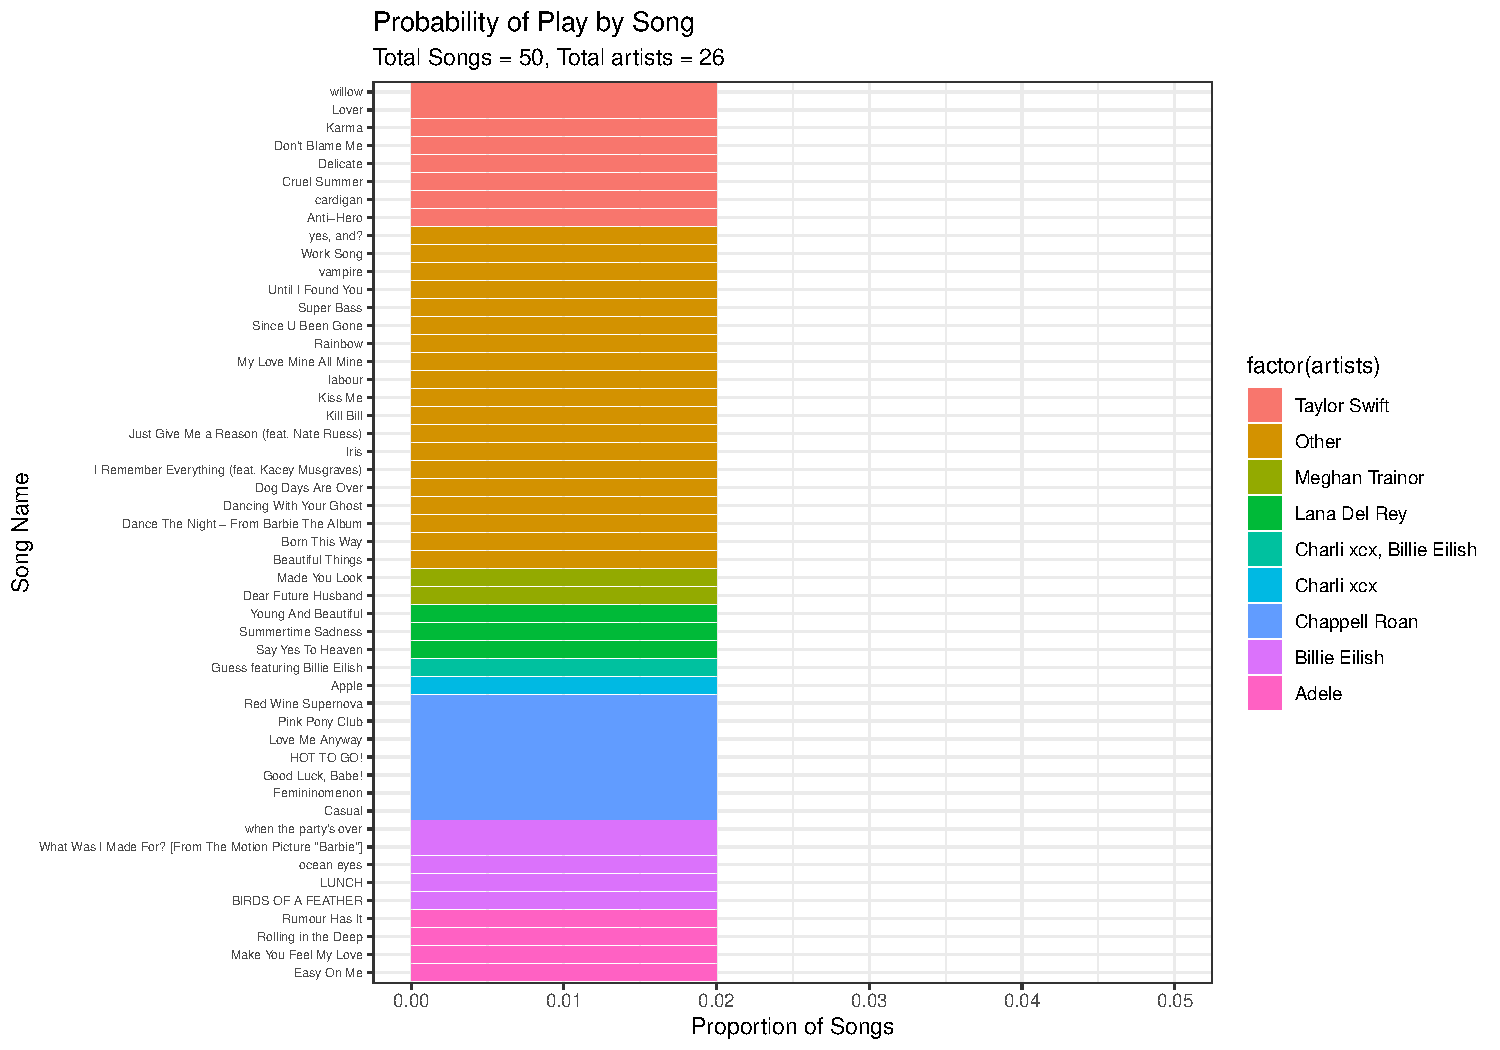
\includegraphics{class10_files/figure-beamer/unnamed-chunk-3-1.pdf}
\end{frame}

\begin{frame}{Population proportions by artist for sampling WITH
replacement}
\phantomsection\label{population-proportions-by-artist-for-sampling-with-replacement}
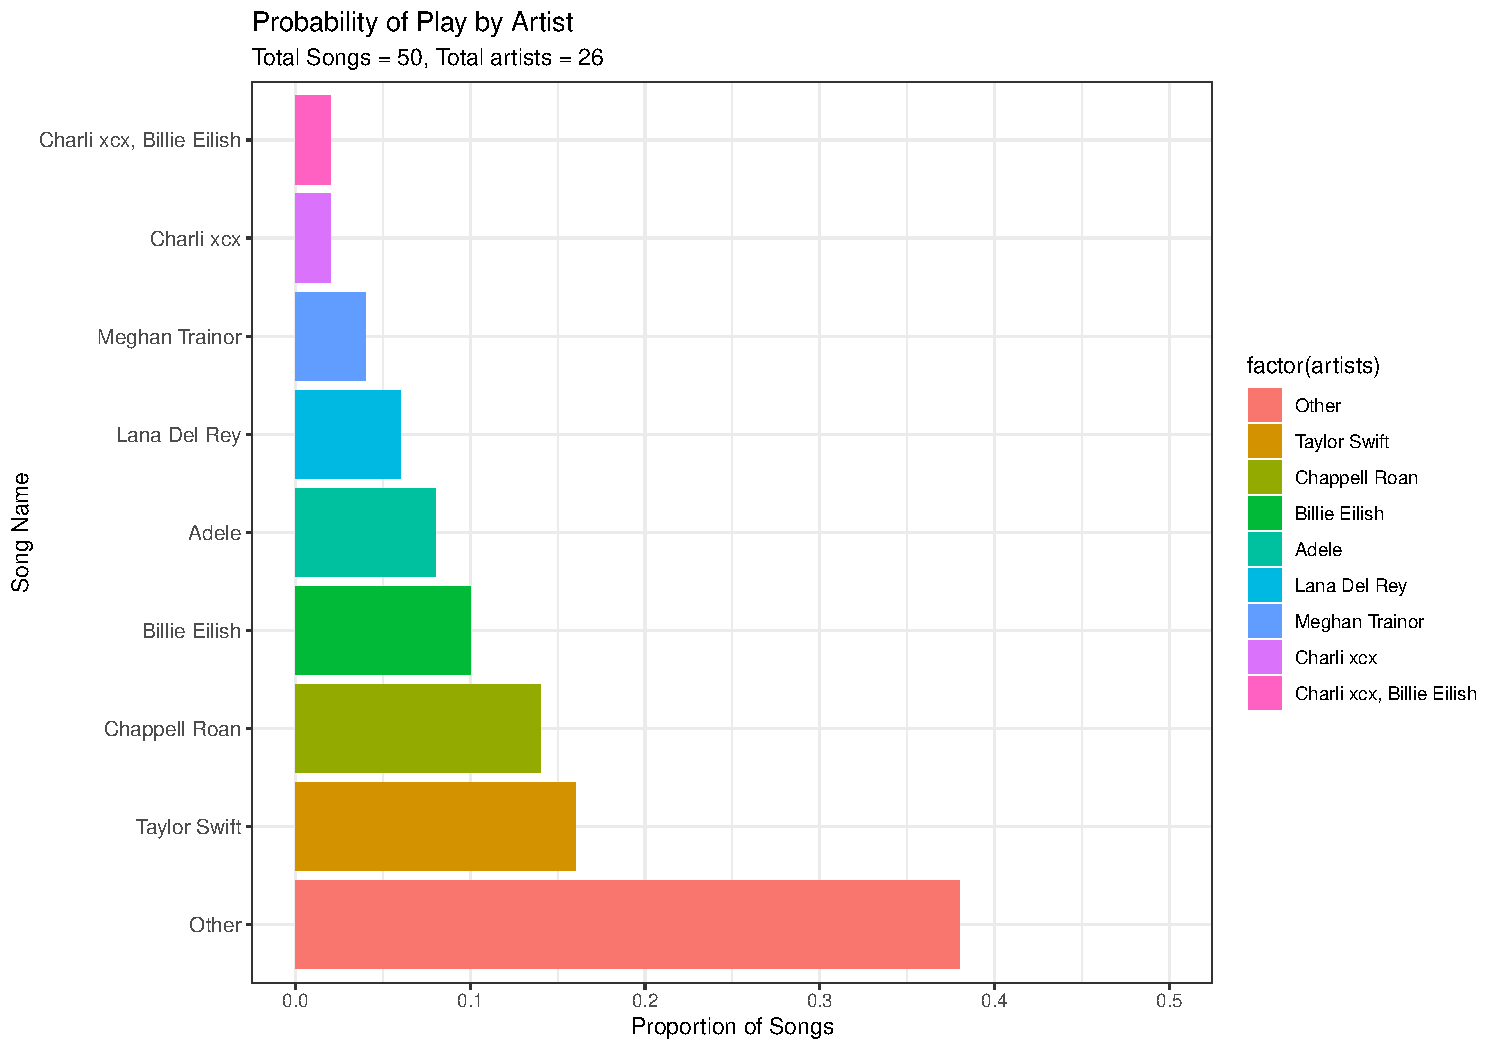
\includegraphics{class10_files/figure-beamer/unnamed-chunk-4-1.pdf}
\end{frame}

\begin{frame}{Drawing the sample space: 1 outcome}
\phantomsection\label{drawing-the-sample-space-1-outcome}
See board\ldots{}
\end{frame}

\begin{frame}{Calculating probability for a single event}
\phantomsection\label{calculating-probability-for-a-single-event}
\[
\begin{aligned}
\operatorname{P}(\operatorname{Next Song by Chappell Roan})&=\frac{\operatorname{count}(\operatorname{Songs by Chappell Roan})}{\operatorname{count}(\operatorname{All Possible Songs})} \\
&= \frac{7}{50} \\
&= 0.14
\end{aligned}
\]
\end{frame}

\begin{frame}{Describing the sample space: 2 disjoint outcomes}
\phantomsection\label{describing-the-sample-space-2-disjoint-outcomes}
See board\ldots{}
\end{frame}

\begin{frame}{Addition Rule for Disjoint Outcomes}
\phantomsection\label{addition-rule-for-disjoint-outcomes}
Describes the probability of event A or event B occurring
(\(P(A \cup B)\))

\[\operatorname{P}(\operatorname{A or B}) = \operatorname{P}(\operatorname{A}) \times \operatorname{P}(\operatorname{B})\]
\end{frame}

\begin{frame}{Example: Addition Rule for Disjoint Outcomes}
\phantomsection\label{example-addition-rule-for-disjoint-outcomes}
See board\ldots{}
\end{frame}

\begin{frame}{\emph{General} Addition Rule for \emph{Non-Disjoint}
Outcomes}
\phantomsection\label{general-addition-rule-for-non-disjoint-outcomes}
Describes the probability of event A or event B occurring

\[\operatorname{P}(\operatorname{A or B}) = \operatorname{P}(\operatorname{A}) \times \operatorname{P}(\operatorname{B}) - \operatorname{P}(\operatorname{A and B})\]
\end{frame}

\begin{frame}{Example: General Addition Rule for Non-Disjoint Outcomes}
\phantomsection\label{example-general-addition-rule-for-non-disjoint-outcomes}
See board\ldots{}
\end{frame}

\begin{frame}{Independent Processes}
\phantomsection\label{independent-processes}
\begin{itemize}
\item
  Two \textbf{\emph{random processes}} are \textbf{\emph{independent}}
  if the outcome of process A provides no information about process B

  \begin{itemize}
  \item
    You roll a die once and get a 3. You still don't know what number
    you'll roll next.
  \item
    You aren't more likely to land on heads when flipping a coin just
    because you also got heads on your last one.
  \end{itemize}
\end{itemize}
\end{frame}

\begin{frame}{Example: Independent Processes with ``True'' Shuffle}
\phantomsection\label{example-independent-processes-with-true-shuffle}
What if we listened to 2 songs in a row using ``true'' shuffle
(i.e.~sampling with replacement)?

Each song goes back into the ``pot'' after it is played and can be
repeated.

What happens to the sample space after the first song?

The sample space does \textbf{\emph{not}} change between events.
\end{frame}

\begin{frame}{Defining the Sample Space}
\phantomsection\label{defining-the-sample-space}
See board\ldots{}
\end{frame}

\begin{frame}{What is the probability we hear a song by Chappell Roan
twice in a row?}
\phantomsection\label{what-is-the-probability-we-hear-a-song-by-chappell-roan-twice-in-a-row}
\begin{itemize}
\item
  7 opportunities for song 1 to be by Chappell Roan
\item
  7 opportunities for song 2 to be by chappell roan
\end{itemize}

\(7 \times 7 = 49 \operatorname{possibilities!}\)

\begin{itemize}
\item
  50 possible songs for song 1
\item
  50 possible songs for song 2
\end{itemize}

\(50 \times 50 = 2500 \operatorname{possibilities!}\)

\(\operatorname{P}(\operatorname{A and B})=\frac{7 \times 7}{50 \times 50}\)
\end{frame}

\begin{frame}{Multiplication Rule for Independent Processes}
\phantomsection\label{multiplication-rule-for-independent-processes}
Describes the probability of event A and event B occurring

\[
\operatorname{P}(\operatorname{A and B})=\operatorname{P}(\operatorname{A}) \times \operatorname{P}(\operatorname{B})
\]
\end{frame}

\begin{frame}{Dependent Processes}
\phantomsection\label{dependent-processes}
\begin{itemize}
\item
  Two \textbf{\emph{random processes}} are \textbf{\emph{dependent}} if
  the probability of process B changes based on the outcome of process A

  \begin{itemize}
  \item
    You're playing poker and cards are about to be dealt. The
    probability that you will receive an Ace changes as each card is
    distributed.
  \item
    The chances that you'll bring an umbrella with you when you leave
    the house changes depending on whether or not its raining.
  \end{itemize}
\end{itemize}
\end{frame}

\begin{frame}{Sampling WITHOUT Replacement}
\phantomsection\label{sampling-without-replacement}
\begin{figure}[H]

{\centering \includegraphics{class10_files/mediabag/Sampling-Without-Rep.png}

}

\caption{\textbf{\emph{Sampling without replacement}} is like drawing a
card from a deck, then drawing another card without putting the first
one back. Repetition is NOT possible.}

\end{figure}%
\end{frame}

\begin{frame}{Example: Dependent Processes with Spotify Shuffle}
\phantomsection\label{example-dependent-processes-with-spotify-shuffle}
What if we listened to 2 songs in a row using Spotify's shuffle
(i.e.~sampling without replacement)

Song does NOT go back into the ``pot'' after it is played and CANNOT be
repeated.

The sample space \textbf{\emph{does}} change between events.
\end{frame}

\begin{frame}{Defining the Sample Space for Dependent Processes}
\phantomsection\label{defining-the-sample-space-for-dependent-processes}
See board\ldots{}
\end{frame}

\begin{frame}{What is the probability we hear a song by Chappell Roan
twice in a row?}
\phantomsection\label{what-is-the-probability-we-hear-a-song-by-chappell-roan-twice-in-a-row-1}
\begin{itemize}
\item
  7 opportunities for song 1 to be by Chappell Roan
\item
  6 opportunities for song 2 to be by chappell roan
\end{itemize}

\(7 \times 6 = 42 \operatorname{possibilities!}\)

\begin{itemize}
\item
  50 possible songs for song 1
\item
  49 possible songs for song 2
\end{itemize}

\(50 \times 49 = 2450 \operatorname{possibilities!}\)

\(\operatorname{P}(\operatorname{A and B})=\frac{7 \times 6}{50 \times 49}\)
\end{frame}

\begin{frame}{General Multiplication Rule for Dependent Processes}
\phantomsection\label{general-multiplication-rule-for-dependent-processes}
Describes the probability of event B occurring given that event A has
already occurred

\[
\operatorname{P}(\operatorname{A and B})=\operatorname{P}(\operatorname{A}) \times \operatorname{P}(\operatorname{B given A})
\] \#\# Distinguishing Independent and Dependent Processes

When processes are independent,
\(\operatorname{P}(\operatorname{A and B})=\operatorname{P}(\operatorname{A}) \times \operatorname{P}(\operatorname{B})\).

If
\(\operatorname{P}(\operatorname{A and B})\ne\operatorname{P}(\operatorname{A}) \times \operatorname{P}(\operatorname{B})\),
the processes are NOT independent.
\end{frame}

\begin{frame}{Probability Density Functions}
\phantomsection\label{probability-density-functions}
\begin{itemize}
\item
  \textbf{\emph{Probability Mass Function:}} categorical
\item
  \textbf{\emph{Probabiity Density Function:}} numerical
\end{itemize}
\end{frame}



\end{document}
